\chapter{Latent Variable Models}
\section{Motivation of Latent Variable Models}
\label{sec:intro_motivation}

Let's say we want to classify some data. If we had access to a corresponding latent variable for each observation \( \mathbf{x}_i \), modeling would be more straightforward. To illustrate this, consider the challenge of finding the latent variable (\ie the true class of \( \mathbf{x} \)) \( z^* = \argmax_{z} p(\mathbf{x} | z) \), as shown in \Cref{fig:clusters}(b).

\begin{figure}[h]
	\begin{center}			
		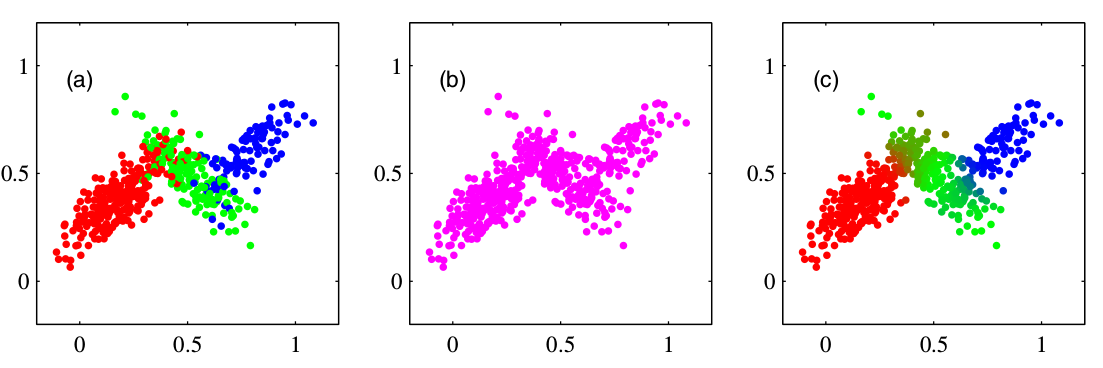
\includegraphics[scale=0.25]{./images/generative/latent.png}
	\end{center}
	\caption{(a) Complete dataset \( p(\mathbf{x} | z) \). (b) Incomplete dataset \( p(\mathbf{x}) \). (c) Inference result.}
	\label{fig:clusters}
\end{figure}

Consider modeling the complete data set \( p(\mathbf{x} | z) \) under the assumption that the observations are independent and identically distributed (i.i.d.). Based on the \Cref{fig:clusters}(a), the joint distribution for a single observation \( (\mathbf{x}_i, \mathbf{z}_i) \) given the model parameters \( \boldsymbol{\theta} \) can be expressed:

\[
p(\mathbf{x}_i, \mathbf{z}_i | \boldsymbol{\theta}) = 
\begin{cases}
p(\mathcal{C}_1) p(\mathbf{x}_i | \mathcal{C}_1) & \text{if } z_i = 0 \\
p(\mathcal{C}_2) p(\mathbf{x}_i | \mathcal{C}_2) & \text{if } z_i = 1 \\
p(\mathcal{C}_3) p(\mathbf{x}_i | \mathcal{C}_3) & \text{if } z_i = 2 \\
\end{cases}
\]



Given \( N \) observations, the joint distribution for the entire dataset \( \{ \mathbf{x}_1, \mathbf{x}_2, \ldots, \mathbf{x}_N \} \) along with their corresponding latent variables \( \{ \mathbf{z}_1, \mathbf{z}_2, \ldots, \mathbf{z}_N \} \) is:

\[
p(\mathbf{x}_1, \mathbf{x}_2, \ldots, \mathbf{x}_N, \mathbf{z}_1, \mathbf{z}_2, \ldots, \mathbf{z}_N | \boldsymbol{\theta}) = \prod_{n=1}^{N} \prod_{k=1}^{K} \pi_k^{z_{nk}} \mathcal{N}(\mathbf{x}_n | \boldsymbol{\mu}_k, \boldsymbol{\Sigma}_k)^{z_{nk}}
\]

Here, \( \pi_k = p(\mathcal{C}_k) \) represents the prior probability of the \( k \)-th component, and \( p(\mathbf{x}_n | \mathcal{C}_k) = \mathcal{N}(\mathbf{x}_n | \boldsymbol{\mu}_k, \boldsymbol{\Sigma}_k) \) denotes the Gaussian distribution associated with component \( \mathcal{C}_k \). Also, \(z_{nk}\in\{0,1\}\) and \(\sum_k z_{nk}=1\).

However, in practice, the latent variables \( \mathbf{z}_k \) are often not directly observable, which complicates the modeling process.

In the following sections, we present various methods for identifying and handling these latent variables to improve the classification and modeling of data.


